\documentclass{beamer}

\usepackage{amsmath}

\usetheme{AnnArbor}
\usecolortheme{crane}
\usefonttheme[onlymath]{serif}

\title{Deep Learning - Foundations and Concepts}
\subtitle{Chapter 7. Gradient Descent}
\author{nonlineark@github}
\date{\today}

\begin{document}

\begin{frame}
    \titlepage
\end{frame}

\begin{frame}
    \frametitle{Outline}
    \tableofcontents
\end{frame}

\section{Error Surfaces}

\begin{frame}
    \frametitle{Gradient and stationary points}
    \begin{block}{Theorem}
        Let the function $f:\mathbb{R}^{n}\to\mathbb{R}$ be differentiable at $a\in\mathbb{R}^{n}$:
        \begin{enumerate}
            \item Near $a$ the function $f$ increases fastest in the direction of $\nabla{}f(a)\in\mathbb{R}^{n}$.
            \item The rate of increase in $f$ is measured by the length of $\nabla{}f(a)$.
            \item If $f$ has a local extremum at $a$ then $\nabla{}f(a)=0$.
        \end{enumerate}
    \end{block}
    \begin{block}{Definition}
        Let $f:\mathbb{R}^{n}\to\mathbb{R}$ be differentiable at $a\in\mathbb{R}^{n}$. Then $a$ is said to be a stationary point for $f$ if $Df(a)=0$, or, equivalently, $\nabla{}f(a)=0$.
    \end{block}
\end{frame}

\begin{frame}
    \frametitle{Gradient and stationary points}
    It's easy to see the correctness of the theorem. Since the rate of increase of $f$ at the point $a$ in an arbitray direction $v\in\mathbb{R}^{n}$ is given by the directional derivative at $v$, we have:
    \begin{equation*}
        |Df(a)v|=|v^{T}\nabla{}f(a)|\le||\nabla{}f(a)||||v||
    \end{equation*}
    where we have used the Cauchy-Schwarz inequality. The rate of increase is maximal if $v$ is a positive scalar multiple of $\nabla{}f(a)$. For the third claim, let's define $g_{j}$ as:
    \begin{equation*}
        g_{j}(t)=f(a_{1},\hdots,a_{j-1},t,a_{j+1},\hdots,a_{n})
    \end{equation*}
    then $g'_{j}(a_{j})=D_{j}f(a)$. Since $f$ has a local extremum at $a$, $g_{j}$ also has a local extremum at $a_{j}$. Thus $g'_{j}(a_{j})=0$ for $1\le{}j\le{}n$, and we have $\nabla{}f(a)=0$.
\end{frame}

\begin{frame}
    \frametitle{Gradient and stationary points}
    During training, we want to optimize the weights and biases $w\in\mathbb{R}^{W}$ by using a chosen error function $E(w)$. From the previous theorem we see that, its smallest value will occur at a point in weight space such that:
    \begin{equation*}
        \nabla{}E(w)=0
    \end{equation*}
    But:
    \begin{itemize}
        \item Global minimum vs. local minimum.
        \item For any point $w$ that is a local minimum, there will generally be other points in weight space that are equivalent minima (weight-space symmetries).
    \end{itemize}
\end{frame}

\begin{frame}
    \frametitle{Local quadratic approximation}
    \begin{block}{Threorem}
        Let $U$ be a convex open subset of $\mathbb{R}^{n}$ and let $a\in{}U$ be a stationary point for $f\in{}C^{2}(U)$. Then we have the following assertions:
        \begin{enumerate}
            \item If $Hf(a)$ is positive definite, then $f$ has a local strict minimum at $a$.
            \item If $Hf(a)$ is negative definite, then $f$ has a local strict maximum at $a$.
        \end{enumerate}
        where $Hf(a)$ is the Hessian of $f$ at $a$.
    \end{block}
\end{frame}

\begin{frame}
    \frametitle{Local quadratic approximation}
    We only prove the first claim. Using Taylor expansion, we see that:
    \begin{align*}
        f(a+h)&=f(a)+h^{T}\nabla{}f(a)+\frac{1}{2}h^{T}Hf(a)h+R_{2}(a,h) \\
        &=f(a)+\frac{1}{2}h^{T}Hf(a)h+R_{2}(a,h)
    \end{align*}
    where $\lim_{h\to{}0}\frac{R_{2}(a,h)}{||h||^{2}}=0$. Since $f\in{}C^{2}(U)$, $Hf(a)$ is a self-adjoint operator. Let $\lambda$ be its smallest eigenvalue. Because $Hf(a)$ is positive definite, $\lambda>0$. Notice that:
    \begin{itemize}
        \item $h^{T}Hf(a)h\ge\lambda||h||^{2}$.
        \item There is $\delta>0$, such that $\frac{|R_{2}(a,h)|}{||h||^{2}}<\frac{\lambda}{4}$ for $||h||<\delta$.
    \end{itemize}
    For $||h||<\delta$, we have:
    \begin{equation*}
        f(a+h)-f(a)=\frac{1}{2}h^{T}Hf(a)h+R_{2}(a,h)>\frac{\lambda}{2}||h||^{2}-\frac{\lambda}{4}||h||^{2}=\frac{\lambda}{4}||h||^{2}
    \end{equation*}
\end{frame}

\begin{frame}
    From the previous theorem, we see that: A necessary and sufficient condition for $w^{*}$ to be a local minimum of the error function $E(w)$ is that the gradient of $E(w)$ should vanish at $w^{*}$ and the Hessian matrix evaluated at $w^{*}$ should be positive definite.
    \begin{figure}
        \caption{Geometry of the error surface in the neighbourhood of a minimum $w^{*}$}
        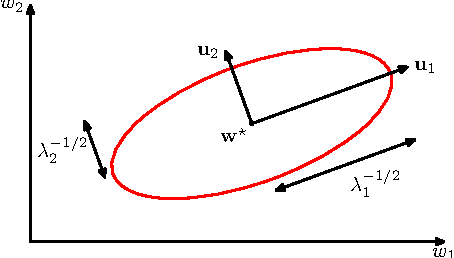
\includegraphics{Figure_2.pdf}
    \end{figure}
\end{frame}

\end{document}